\documentclass[a4paper,11pt]{article}

% =====================================================================
% 1. ENCODAGE, POLICES ET LANGUE
% =====================================================================
\usepackage[utf8]{inputenc}       % Gestion de l'UTF-8
\usepackage[T1]{fontenc}          % Encodage des caractères pour le français
\usepackage[french]{babel}        % Support du français
\usepackage{lmodern}              % Police propre et vectorielle
\usepackage{gensymb}

% =====================================================================
% 2. MISE EN PAGE ET GÉOMÉTRIE
% =====================================================================
\usepackage[a4paper, margin=3.2cm, top=3.5cm, bottom=4cm]{geometry}
\usepackage{setspace}             % Gestion de l'interligne
\usepackage{fancyhdr}             % En-têtes et pieds de page personnalisés (Remplace fancyheadings)
\usepackage{lastpage}             % Pour obtenir le numéro de la dernière page (\pageref{LastPage})
\usepackage[absolute,overlay]{textpos} % Positionnement absolu de blocs de texte
\usepackage{eso-pic}              % Pour ajouter des éléments en arrière-plan de la page

% =====================================================================
% 3. MATHÉMATIQUES ET SCIENCES
% =====================================================================
\usepackage{amsmath}              % Commandes mathématiques de base
\usepackage{amsfonts}             % Polices mathématiques
\usepackage{amssymb}              % Symboles mathématiques
\usepackage{siunitx}              % Alignement et écriture des unités scientifiques

% =====================================================================
% 4. GRAPHIQUES, TRACÉS ET DIAGRAMMES
% =====================================================================
\usepackage{graphicx}             % Inclusion d'images
\graphicspath{{Param/}, {Images/}} % Dossiers où chercher les images

\usepackage{tikz}                 % Dessin vectoriel personnalisé
\usetikzlibrary{shapes.geometric, arrows, chains, positioning, babel}
\usepackage{pgfplots}             % Tracé de graphiques mathématiques de haute qualité
\pgfplotsset{compat=1.18}

\usepackage[european, straightvoltages, RPvoltages]{circuitikz} % Tracé de circuits électriques

% =====================================================================
% 5. TABLEAUX
% =====================================================================
\usepackage{booktabs}             % Tableaux de qualité professionnelle (\toprule, \midrule, etc.)
\usepackage{tabularx}             % Tableaux à largeur fixe adaptative
\usepackage{array}                % Personnalisation avancée des colonnes
\usepackage{longtable}            % Tableaux multipages
\usepackage{makecell}             % Retours à la ligne et mise en forme dans les cellules
\usepackage{rotating}             % Pour tourner les tableaux ou les figures (mode paysage local)

% =====================================================================
% 6. STRUCTURATION, BLOCS ET COULEURS
% =====================================================================
\usepackage[table]{xcolor}        % Gestion des couleurs et coloration des lignes de tableaux
\usepackage{titlesec}             % Personnalisation des titres (\section, \subsection)
\usepackage{enumitem}             % Personnalisation des listes à puces
\usepackage{subcaption}           % Légendes pour les sous-figures
\usepackage{float}                % Forcer le positionnement des éléments graphiques ([H])
\usepackage{listings}             % Inclusion et coloration de code source (Python, C++, etc.)
\usepackage[most]{tcolorbox}      % Boîtes d'alerte et encadrés stylisés
\usepackage{pifont}               % Symboles et puces spécifiques (\ding)
\usepackage{lipsum}               % Générateur de faux texte de test

% =====================================================================
% 7. LIENS HYPERTEXTES (Toujours charger en dernier !)
% =====================================================================
\usepackage[hidelinks]{hyperref}  % Liens cliquables internes et externes sans bordures rouges


\hypersetup{
    colorlinks=true,
    linkcolor=blue,
    citecolor=blue,
    urlcolor=blue,
    pdftitle={Rapport de projet},
    pdfauthor={Auteur},
    pdfkeywords={projet, rapport}
}

\begin{document}

\begin{titlepage}
    \centering

    % --- Logo en haut ---
    
\includegraphics[width=0.9\linewidth]{Param/Polytech_Univ.png}\\[1.5cm]

    % --- Titre principal ---
    {\Huge \textbf{Rapport de conception SoC Contrôleur I2C}}\\[0.5cm]
    \rule{0.7\textwidth}{0.5pt}\\[0.8cm]
    {\Large \textbf{ETN4 - SETR}}\\[1cm]
    
    % --- Mise en page en deux colonnes (élève / encadrants) ---
    \noindent
    \begin{minipage}[t]{0.48\textwidth}
        \raggedright
        {\large \textbf{Élèves :}}\\[0.3cm]
        {\large
        Nolan \textsc{BUCHET}}\\[0.6cm]
        {\large
        Maxence \textsc{BOULEAU}}\\[0.6cm]
    \end{minipage}%
    \hfill
    \begin{minipage}[t]{0.48\textwidth}
        \raggedleft
        {\large \textbf{Date :}}\\[0.3cm]
        {\large
        Octobre 2026}
    \end{minipage}
    \vfill
\end{titlepage}

% LOGO IUT
\AddToHook{shipout/background}{%
  \begin{textblock*}{100cm}(100cm,100cm) % Ajustez les coordonnées pour décaler l'image
  \begin{tikzpicture}[remember picture, overlay]
    \node[anchor=north east, inner sep=18pt] at (current page.north east) {%
      
\includegraphics[scale=0.18]{Logo_Universite_de_nantes.png}%
    };
  \end{tikzpicture}%
  \end{textblock*}
}


\AddToHook{shipout/background}{%
  \begin{textblock*}{100cm}(100cm,100cm) % Ajustez '15cm' pour déplacer l'image plus à droite
    \begin{tikzpicture}[remember picture, overlay]
      \node[anchor=north west, inner sep=25pt] at (current page.north west) {%
        
\includegraphics[scale=0.50]{logo_poly.png}%
      };
    \end{tikzpicture}%
  \end{textblock*}
}


% NOM FICHIER
\AddToHook{shipout/background}{%
  \begin{textblock*}{1cm}(1cm,1cm)
  \end{textblock*}
  \begin{tikzpicture}[remember picture, overlay]
    \node[anchor=north, inner sep=50pt] at (current page.north) {%    
    {\fontsize{10}{13}\selectfont Rapport de conception du controleur I2C}
    };
  \end{tikzpicture}%
}

% PAGE
\AddToHook{shipout/background}{%
  \begin{textblock*}{1cm}(1cm,1cm)
  \end{textblock*}
  \begin{tikzpicture}[remember picture, overlay]
    \node[anchor=south, inner sep=50pt] at (current page.south) {%
    \thepage/\pageref{LastPage}
    };
  \end{tikzpicture}%
}

% NOM PRENOM
\AddToHook{shipout/background}{%
  \begin{textblock*}{1cm}(1cm,1cm)
  \end{textblock*}
  \begin{tikzpicture}[remember picture, overlay]
    \node[anchor=south west, inner sep=50pt] at (current page.south west) {%    
    {\fontsize{10}{13}\selectfont Maxence BOULEAU \& Nolan BUCHET}
    };
  \end{tikzpicture}%
}

% DATE
\AddToHook{shipout/background}{%
  \begin{textblock*}{1cm}(1cm,1cm)
  \end{textblock*}
  \begin{tikzpicture}[remember picture, overlay]
    \node[anchor=south east, inner sep=50pt] at (current page.south east) {%    
    {\fontsize{10}{13}\selectfont Octobre 2026}
    };
  \end{tikzpicture}%
}


\setlength{\headheight}{14pt}
\pagestyle{fancy}

\fancyhead[L]{\large} % Left side of the header (section title)
\fancyhead[R]{\large} % Right side of the header (page number)

% Footer configuration
\fancyfoot[C]{\large} % Centered text in the footer

\renewcommand{\headrulewidth}{1pt} % Header rule thickness
\renewcommand{\footrulewidth}{1pt} % Footer rule thickness




\tableofcontents

\newpage

\section{Contexte}

Ce rapport s'inscrit dans l'étude de cas E2 « Conception de SoC » du département ETN de Polytech Nantes (ETN5, semestre 9). L'étude de cas consiste à constituer un groupe de concepteurs qui développe, par binômes, les différents composants d'un système sur puce (SoC) afin d'aller le plus loin possible dans sa réalisation.
\\

\section{Introduction}

L'I2C est une liaison série synchrone à deux fils, SCL pour l'horloge et SDA pour les données, très répandue pour relier un processeur à des capteurs, des mémoires ou des convertisseurs. 
\\

Ce document présente la conception d'un contrôleur I2C fonctionnant en mode maître. Le circuit génère l'horloge SCL et les conditions START et STOP, émet l'adresse de l'esclave, puis envoie ou reçoit jusqu'à 8 octets avec gestion des acquittements. 
La démarche suit le plan imposé par l'étude de cas, du besoin jusqu'au circuit :
\\

\begin{itemize}
    \item Le cahier des charges
    \item Les spécifications
    \item La conception
    \item La description VHDL et la synthèse
    \item Le bilan
\end{itemize}


\section{Cadhier des charges}

\subsection{Objectif du circuit}

Le contrôleur I2C a pour rôle d'assurer le couplage du processeur avec son
environnement extérieur via une liaison série de type I2C (signaux SCL et SDA). Il
fonctionne en mode maître : il génère l'horloge SCL, les conditions START et STOP, émet
l'adresse de l'esclave, puis émet ou reçoit une suite d'octets selon la configuration
programmée par le processeur.
\\

\subsection{Fonctionnalités attendues}

Les fonctions de service du circuit sont :
\\

\begin{itemize}
    \item Le circuit peut être configuré par le processeur, la configuration porte sur :
    \begin{enumerate}
        \item la vitesse de transmission : 100 kbit/s (mode standard) ou 400 kbit/s (mode rapide),
        \item la génération d'une interruption en fin de transaction (avec ou sans),
        \item le sens du transfert : écriture (maître vers esclave) ou lecture (esclave vers maître),
        \item le nombre d'octets de données à transmettre ou à recevoir (de 1 à 8),
        \item l'adresse de l'esclave visé (7 bits).
    \end{enumerate}
    \item Le circuit peut émettre une trame I2C : START, adresse + bit R/W, octets de données avec acquittement, STOP.
    \item Le circuit peut recevoir une suite d'octets en provenance de l'esclave, acquitter chaque octet (ACK) et refuser le dernier (NACK) avant le STOP.
    \item Le circuit détecte l'absence d'acquittement de l'esclave (NACK) et le signale dans le registre de statut.
    \item Le circuit supporte l'étirement d'horloge (clock stretching) imposé par un esclave.
    \item Le circuit peut générer une interruption à l'issue d'une transaction, selon la configuration faite.
\end{itemize}

\subsection{Utilisation du circuit}

Le circuit est utilisé au sein du système sur puce de l'étude de cas,
connecté au bus 16 bits du processeur. Le schéma de câblage du circuit à concevoir est le
suivant :
\\

\begin{figure}[H]
    \centering
    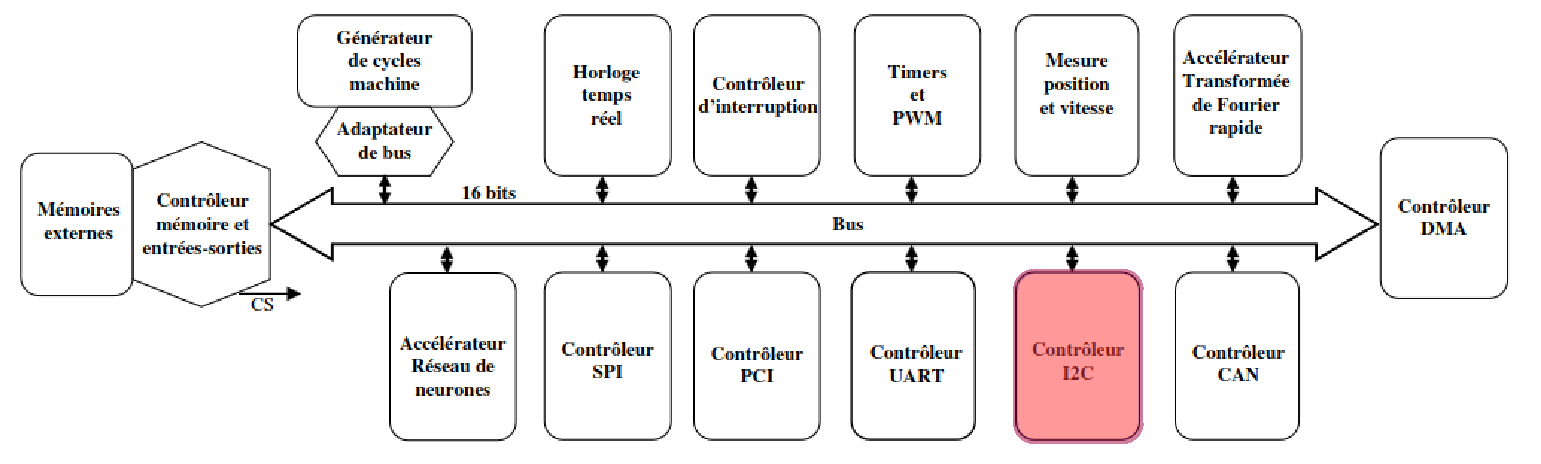
\includegraphics[width=0.95\linewidth]{Images/1_CDC/Architecture.pdf}
    \caption{Architecture du système sur puce considéré}
\end{figure}

Le schéma de câblage du circuit à concevoir est le suivant :
\\

\begin{figure}[H]
    \centering
    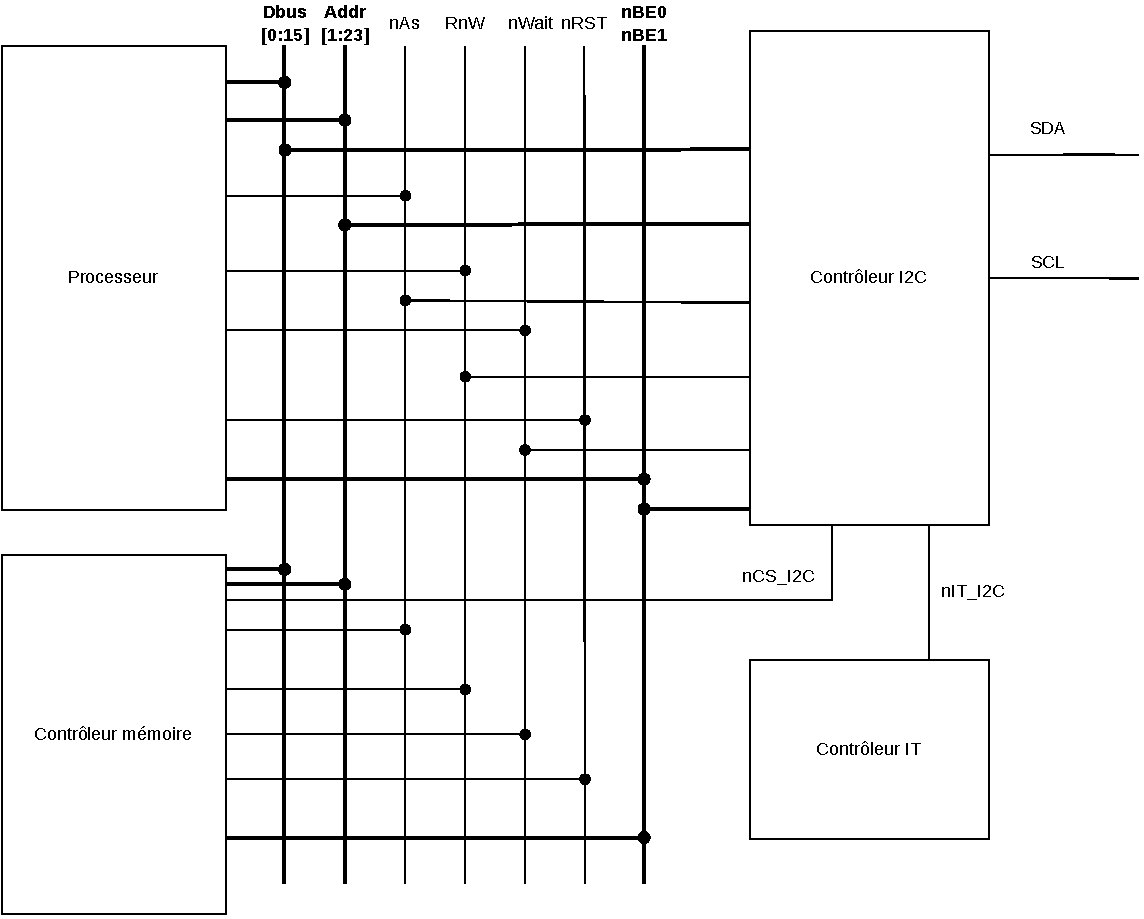
\includegraphics[width=0.95\linewidth]{Images/1_CDC/Schema_cablage.pdf}
    \caption{Schéma de câblage du circuit I2C}
\end{figure}

Les signaux logiques d'entrée-sortie du composant sont résumés dans le tableau suivant
(sens indiqué du point de vue du contrôleur I2C).
\\

\begin{table}[H]
    \centering
    \begin{tabularx}{\textwidth}{|c|c|X|}
        \hline
        \textbf{Nom du signal} & \textbf{Sens} & \textbf{Description} \\
        \hline
        DBus & bidirectionnel & Données codées sur 16 bits, bus de données du processeur \\
        \hline
        Addr & entrée & Données codées sur 22 bits, bus d'adresse du processeur \\
        \hline
        nAS & entrée & Address Strobe, valide la présence d'une adresse sur le bus \\
        \hline
        RnW & entrée & Read not Write, sélection lecture ou écriture \\
        \hline
        nWAIT & entrée & Insertion de cycles d'attente (non utilisé dans le cas du contrôleur I2C : tous les transferts se font en 1 cycle) \\
        \hline
        nRST & entrée & not Reset, signal d'initialisation du circuit \\
        \hline
        CLK & entrée & Clock, horloge du circuit \\
        \hline
        nBE0--nBE1 & entrée & Byte Enable, ordre des octets sur le bus de données \\
        \hline
        nCS\_I2C & entrée & Chip Select, sélection du contrôleur I2C (produit par le contrôleur mémoire et E/S) \\
        \hline
        nIT\_I2C & sortie & Interrupt, signal d'interruption vers le processeur \\
        \hline
        SCL & sortie & Horloge de la liaison I2C \\
        \hline
        SDA & bidirectionnel & Données de la liaison I2C \\
        \hline
    \end{tabularx}
    \caption{Signaux logiques d'entrée-sortie du contrôleur I2C}
\end{table}

\subsection{Chronogrammes caractéristiques}

Cycles d'échange avec le processeur. Les cycles de lecture et d'écriture sont ceux du
bus : synchrone sur CLK, transfert en 1 cycle,
nAS et nBE0-nBE1 actifs pendant le cycle, RnW à 1 pour une lecture et à 0 pour une
écriture. Les écritures concernent la configuration, l'adresse esclave et les données à
émettre ; les lectures concernent le statut et les données reçues.
\\

\begin{figure}[H]
    \centering
    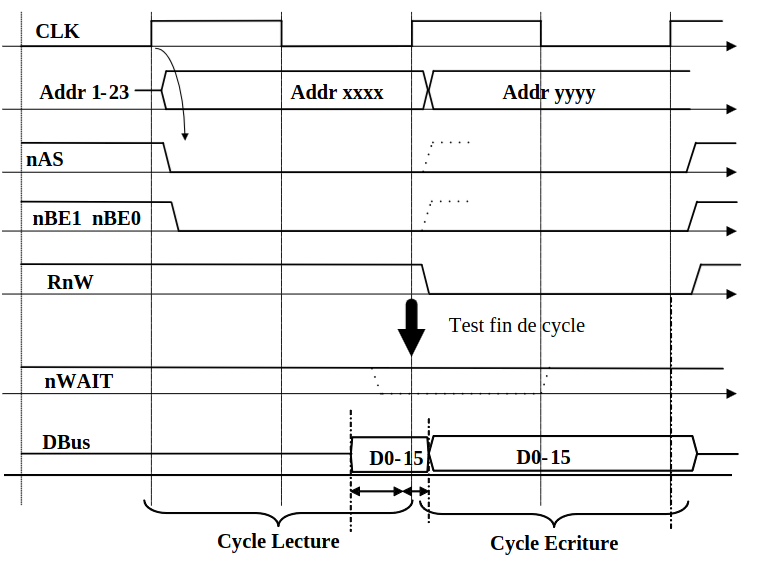
\includegraphics[width=0.95\linewidth]{Images/1_CDC/Cycle_cours.png}
    \caption{Chronogramme des cycles d'échange}
\end{figure}

Les cycles d'écriture permettent soit de configurer les registres du contrôleur I2C, soit d'envoyer des données à transmettre sur la ligne série.
\\

Les cycles de lecture servent soit à consulter les registres d'état du contrôleur, soit à récupérer les données reçues via la liaison série.
\\

La figure suivante illustre le format des trames de données émises et reçues sur le bus série.
\\

\begin{figure}[H]
    \centering
    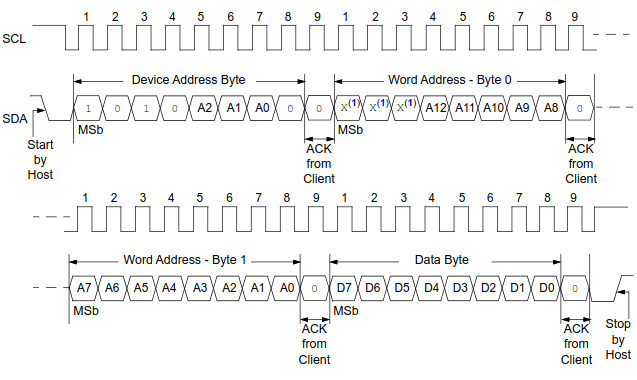
\includegraphics[width=0.95\linewidth]{Images/1_CDC/Trame_I2C_W.png}
    \caption{Chronogramme des trames I2C - Ecriture}
\end{figure}

\begin{figure}[H]
    \centering
    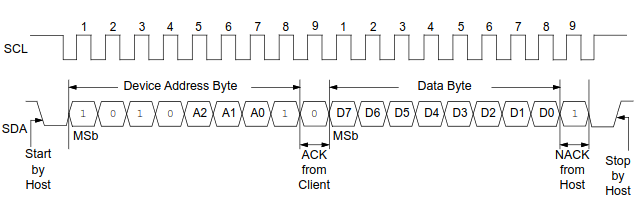
\includegraphics[width=0.95\linewidth]{Images/1_CDC/Trame_I2C_R.png}
    \caption{Chronogramme des trames I2C - Lecture}
\end{figure}

\subsection{Contraintes}

Les contraintes considérées sont celles du projet. Le composant est développé en VHDL
dans l'environnement HDL Designer de Mentor Graphics (saisie, simulation sous
ModelSim, synthèse). Le circuit doit pouvoir être connecté sur le bus imposé, sans
modification de ce dernier, et être réutilisable comme IP.
\\

\section{Spécifications}

\subsection{Caractérisation de l'environement}

L'environnement du circuit est constitué de deux entités :
\\

L'ensemble « \textbf{Système à uP} » formé par le processeur, le contrôleur mémoire et le
contrôleur d'interruptions ;
\\

Un \textbf{esclave I2C} distant (capteur, mémoire, etc.).
\\

L'entité Système à uP peut configurer le contrôleur, écrire l'adresse de l'esclave, écrire les
données à envoyer, lancer une transaction, lire l'état, lire les données reçues et gérer
l'interruption produite. L'entité Esclave distant répond à son adresse, acquitte les octets
reçus, ou émet des octets lorsque le maître lit.
\\

Comportement de l'entité Système à uP (en considérant les cycles de fonctionnement
comme instantanés) : depuis l'état Autre, le processeur évolue selon les événements
suivants :
\\

\begin{figure}[H]
    \centering
    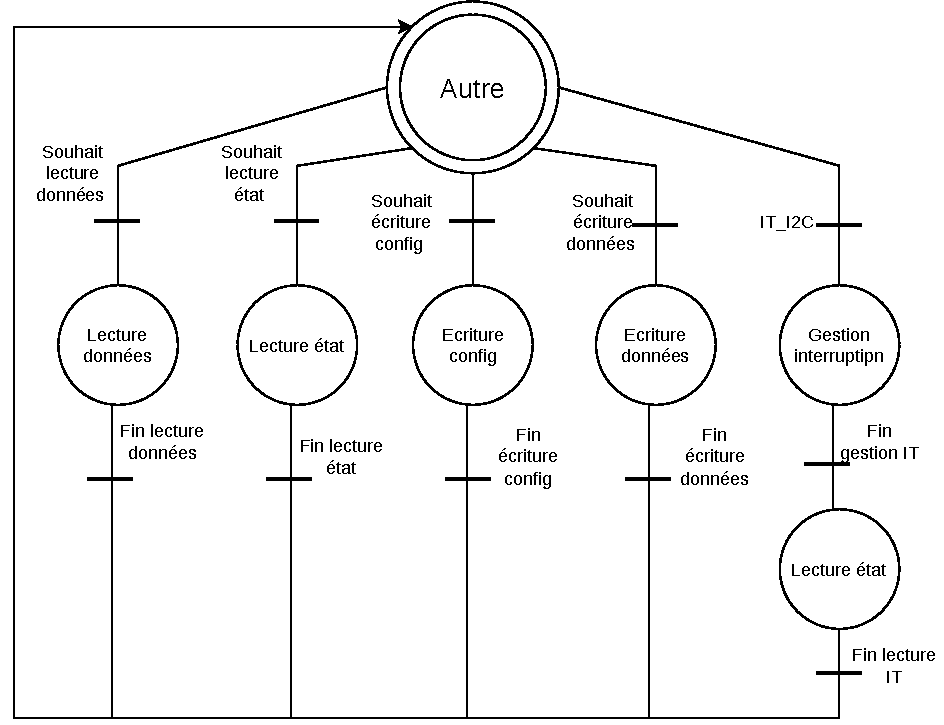
\includegraphics[width=0.95\linewidth]{Images/2_SPEC/Comportement_uc.pdf}
    \caption{Comportement de l'entité Système à uP}
\end{figure}

\section{Conception}

\section{VHDL et synthèse}

\section{Conclusion}

\section{Bibliographie}



\section{Annexes}

\end{document}